\documentclass[12pt]{article}
\usepackage[utf8]{inputenc}
\usepackage{mathtools} % also loads amsmath
\usepackage{amsmath,amsthm,amsfonts,amssymb}
\usepackage{tikz}

% \usepackage{subfig}
\usepackage[english]{babel}
% \usepackage{capt-of}
% \usepackage{tabularray}
\usepackage{caption}
\usepackage{subcaption}
% \usepackage{subcaption}
% \captionsetup{compatibility=false}
\usepackage{graphicx}
\newtheorem{theorem}{Theorem}
\usetikzlibrary{calc}
\usetikzlibrary{shapes}
\usepackage{hyperref}
%might be unnecessary
% \usepackage{doi}

%bibliography CMDS

%\usepackage{cite}
%\usepackage[style=alphabetic]{biblatex}
%\bibliographystyle{plain}

%\usepackage[style=alphabetic]{biblatex}

% \usepackage[backend=biber,style=alphabetic]{biblatex}
\usepackage[backend=biber,style=numeric]{biblatex}
% \usepackage[backend=biber,style=abbrv]{biblatex}
% \usepackage[backend=biber,style=alpha]{biblatex}
%\usepackage[backend=bibtex,style=alphabetic]{biblatex}
\addbibresource{./bibb.bib}

%%% With amsthm package, creates environments for nicely formatted,
%%% labeled, and numbered propositions, etc.
\theoremstyle{plain}

\newtheorem{thm}{Theorem}[section]
\newtheorem{lemma}[thm]{Lemma}
\newtheorem{prop}[thm]{Proposition}
\newtheorem{conj}[thm]{Conjecture}
\newtheorem{cor}[thm]{Corollary}
\newtheorem{claim}[thm]{Claim}
\newtheorem{fact}[thm]{Fact}
\newtheorem{constraint}[thm]{Constraint}
\newtheorem{condition}[thm]{Condition}

\theoremstyle{definition}
\newtheorem{eg}[thm]{Example}
% \newtheorem{defn}[thm]{Definition}
\newtheorem{definition}{Definition}[section]
\newtheorem{rem}[thm]{Remark}
\newtheorem{observ}[thm]{Observation}
\newtheorem{open}[thm]{Open Problem}
\newtheorem{prob.}[thm]{Problem}
\newtheorem{quest}[thm]{Question}

% I used these for making definitions and theorems, not what is above
\theoremstyle{remark}
\newtheorem{remark}[thm]{Remark}
\newtheorem{note}[thm]{Note}

\theoremstyle{definition}
% \newtheorem{definition}{Definition}[section]
\newtheorem{exmp}{Example}[section]

%custom commands

% blank cell
\newcommand{\cell}[4]{ \draw[thick] ( #1 , #2 ) rectangle ( #3 , #4 );}

% invisible cell for spacing
\newcommand{\spacecell}[4]{ \draw[thick, color=white] ( #1 , #2 ) rectangle ( #3 , #4 );}

% open cell 
\newcommand{\cellopen}[4]{ \draw[thick] ( #1 , #2 ) rectangle ( #3 , #4 ); \node[shape=circle,draw=red,fill=red, inner sep=0pt,minimum size=3pt] (A) at ( #1 * 0.5 + #3 * 0.5 , #2 * 0.5 + #4 * 0.5 ){};}

\newcommand{\cellA}[4]{ \draw[thick] ( #1 , #2 ) rectangle ( #3 , #4 ); \draw[red, thick, densely dotted] (#3 * 0.5 + #1 * 0.5 , #2) -- (#1, #4 * 0.5 + #2 * 0.5);}
\newcommand{\cellB}[4]{ \draw[thick] ( #1 , #2 ) rectangle ( #3 , #4 ); \draw[red, thick, densely dotted] (#3 * 0.5 + #1 * 0.5 , #2) -- (#3, #4 * 0.5 + #2 * 0.5);}
\newcommand{\cellC}[4]{ \draw[thick] ( #1 , #2 ) rectangle ( #3 , #4 ); \draw[red, thick, densely dotted] (#3 * 0.5 + #1 * 0.5 , #4) -- (#3, #4 * 0.5 + #2 * 0.5);}
\newcommand{\cellD}[4]{ \draw[thick] ( #1 , #2 ) rectangle ( #3 , #4 ); \draw[red, thick, densely dotted] (#3 * 0.5 + #1 * 0.5 , #4) -- (#1, #4 * 0.5 + #2 * 0.5);}
\newcommand{\cellE}[4]{ \draw[thick] ( #1 , #2 ) rectangle ( #3 , #4 ); \draw[red, thick, densely dotted] (#3, #4 * 0.5 + #2 * 0.5) -- (#1, #4 * 0.5 + #2 * 0.5);}
\newcommand{\cellF}[4]{ \draw[thick] ( #1 , #2 ) rectangle ( #3 , #4 ); \draw[red, thick, densely dotted] (#3 * 0.5 + #1 * 0.5 , #2) -- (#3 * 0.5 + #1 * 0.5 , #4);}

\newcommand{\cellf}[4]{\filldraw[gray!40] ( #1 , #2 ) rectangle ( #3 , #4 ); \draw[thick] ( #1 , #2 ) rectangle ( #3 , #4 );}

\newcommand{\cellAf}[4]{\filldraw[gray!40] ( #1 , #2 ) rectangle ( #3 , #4 ); \draw[thick] ( #1 , #2 ) rectangle ( #3 , #4 ); \draw[red, thick, densely dotted] (#3 * 0.5 + #1 * 0.5 , #2) -- (#1, #4 * 0.5 + #2 * 0.5);}
\newcommand{\cellBf}[4]{\filldraw[gray!40] ( #1 , #2 ) rectangle ( #3 , #4 ); \draw[thick] ( #1 , #2 ) rectangle ( #3 , #4 ); \draw[red, thick, densely dotted] (#3 * 0.5 + #1 * 0.5 , #2) -- (#3, #4 * 0.5 + #2 * 0.5);}
\newcommand{\cellCf}[4]{\filldraw[gray!40] ( #1 , #2 ) rectangle ( #3 , #4 ); \draw[thick] ( #1 , #2 ) rectangle ( #3 , #4 ); \draw[red, thick, densely dotted] (#3 * 0.5 + #1 * 0.5 , #4) -- (#3, #4 * 0.5 + #2 * 0.5);}
\newcommand{\cellDf}[4]{\filldraw[gray!40] ( #1 , #2 ) rectangle ( #3 , #4 ); \draw[thick] ( #1 , #2 ) rectangle ( #3 , #4 ); \draw[red, thick, densely dotted] (#3 * 0.5 + #1 * 0.5 , #4) -- (#1, #4 * 0.5 + #2 * 0.5);}
\newcommand{\cellEf}[4]{\filldraw[gray!40] ( #1 , #2 ) rectangle ( #3 , #4 ); \draw[thick] ( #1 , #2 ) rectangle ( #3 , #4 ); \draw[red, thick, densely dotted] (#3, #4 * 0.5 + #2 * 0.5) -- (#1, #4 * 0.5 + #2 * 0.5);}
\newcommand{\cellFf}[4]{\filldraw[gray!40] ( #1 , #2 ) rectangle ( #3 , #4 ); \draw[thick] ( #1 , #2 ) rectangle ( #3 , #4 ); \draw[red, thick, densely dotted] (#3 * 0.5 + #1 * 0.5 , #2) -- (#3 * 0.5 + #1 * 0.5 , #4);}


% \newcommand{\cellA}[4]{\draw[red, thick, densely dotted] ( #1 + 0.5 , #2 ) arc(0:90:{0.5}); \draw[thick] ( #1 , #2 ) rectangle ( #3 , #4 );}
% \newcommand{\cellB}[4]{\draw[red, thick, densely dotted] ( #1 + 1 , #2 + 0.5 ) arc(90:180:{0.5}); \draw[thick] ( #1 , #2 ) rectangle ( #3 , #4 );}
% \newcommand{\cellC}[4]{\draw[red, thick, densely dotted] ( #1 + 0.5, #2 + 1 ) arc(180:270:{0.5}); \draw[thick] ( #1 , #2 ) rectangle ( #3 , #4 );}
% \newcommand{\cellD}[4]{\draw[red, thick, densely dotted] ( #1 , #2 + 0.5 ) arc(-90:0:{0.5}); \draw[thick] ( #1 , #2 ) rectangle ( #3 , #4 );}
% \newcommand{\cellE}[4]{\draw[red, thick, densely dotted] (#3, #4 * 0.5 + #2 * 0.5) -- (#1, #4 * 0.5 + #2 * 0.5); \draw[thick] ( #1 , #2 ) rectangle ( #3 , #4 );}
% \newcommand{\cellF}[4]{\draw[red, thick, densely dotted] (#3 * 0.5 + #1 * 0.5 , #2) -- (#3 * 0.5 + #1 * 0.5 , #4); \draw[thick] ( #1 , #2 ) rectangle ( #3 , #4 );}
% \newcommand{\cellG}[4]{\draw[red, thick, densely dotted] ( #1 + 0.5 , #2 ) arc(0:90:{0.5}); \draw[red, thick, densely dotted] ( #1 + 0.5, #2 + 1 ) arc(180:270:{0.5}); \draw[thick] ( #1 , #2 ) rectangle ( #3 , #4 );}
% \newcommand{\cellH}[4]{\draw[red, thick, densely dotted] ( #1 , #2 + 0.5 ) arc(-90:0:{0.5}); \draw[red, thick, densely dotted] ( #1 + 1 , #2 + 0.5 ) arc(90:180:{0.5}); \draw[thick] ( #1 , #2 ) rectangle ( #3 , #4 );}
% \newcommand{\cellI}[4]{\draw[red, thick, densely dotted] (#3 * 0.5 + #1 * 0.5 , #2) -- (#3 * 0.5 + #1 * 0.5 , #4); \node[shape=circle,draw=none,fill=white, inner sep=3pt,minimum size=5pt] (A) at ( #1 + 0.5 , #2 + 0.5 ) {}; \draw[red, thick, densely dotted] (#3, #4 * 0.5 + #2 * 0.5) -- (#1, #4 * 0.5 + #2 * 0.5); \draw[thick] ( #1 , #2 ) rectangle ( #3 , #4 );}
% \newcommand{\cellJ}[4]{\draw[red, thick, densely dotted] (#3, #4 * 0.5 + #2 * 0.5) -- (#1, #4 * 0.5 + #2 * 0.5); \node[shape=circle,draw=none,fill=white, inner sep=3pt,minimum size=5pt] (A) at ( #1 + 0.5 , #2 + 0.5 ) {}; \draw[thick] ( #1 , #2 ) rectangle ( #3 , #4 ); \draw[red, thick, densely dotted] (#3 * 0.5 + #1 * 0.5 , #2) -- (#3 * 0.5 + #1 * 0.5 , #4);}

% \newcommand{\cellAf}[4]{\filldraw[gray!40] ( #1 , #2 ) rectangle ( #3 , #4 ); \draw[red, thick, densely dotted] ( #1 + 0.5 , #2 ) arc(0:90:{0.5}); \draw[thick] ( #1 , #2 ) rectangle ( #3 , #4 );}
% \newcommand{\cellBf}[4]{\filldraw[gray!40] ( #1 , #2 ) rectangle ( #3 , #4 ); \draw[red, thick, densely dotted] ( #1 + 1 , #2 + 0.5 ) arc(90:180:{0.5}); \draw[thick] ( #1 , #2 ) rectangle ( #3 , #4 );}
% \newcommand{\cellCf}[4]{\filldraw[gray!40] ( #1 , #2 ) rectangle ( #3 , #4 ); \draw[red, thick, densely dotted] ( #1 + 0.5, #2 + 1 ) arc(180:270:{0.5}); \draw[thick] ( #1 , #2 ) rectangle ( #3 , #4 );}
% \newcommand{\cellDf}[4]{\filldraw[gray!40] ( #1 , #2 ) rectangle ( #3 , #4 ); \draw[red, thick, densely dotted] ( #1 , #2 + 0.5 ) arc(-90:0:{0.5}); \draw[thick] ( #1 , #2 ) rectangle ( #3 , #4 );}
% \newcommand{\cellEf}[4]{\filldraw[gray!40] ( #1 , #2 ) rectangle ( #3 , #4 ); \draw[red, thick, densely dotted] (#3, #4 * 0.5 + #2 * 0.5) -- (#1, #4 * 0.5 + #2 * 0.5); \draw[thick] ( #1 , #2 ) rectangle ( #3 , #4 );}
% \newcommand{\cellFf}[4]{\filldraw[gray!40] ( #1 , #2 ) rectangle ( #3 , #4 ); \draw[red, thick, densely dotted] (#3 * 0.5 + #1 * 0.5 , #2) -- (#3 * 0.5 + #1 * 0.5 , #4); \draw[thick] ( #1 , #2 ) rectangle ( #3 , #4 );}
% \newcommand{\cellGf}[4]{\filldraw[gray!40] ( #1 , #2 ) rectangle ( #3 , #4 ); \draw[red, thick, densely dotted] ( #1 + 0.5 , #2 ) arc(0:90:{0.5}); \draw[red, thick, densely dotted] ( #1 + 0.5, #2 + 1 ) arc(180:270:{0.5}); \draw[thick] ( #1 , #2 ) rectangle ( #3 , #4 );}
% \newcommand{\cellHf}[4]{\filldraw[gray!40] ( #1 , #2 ) rectangle ( #3 , #4 ); \draw[red, thick, densely dotted] ( #1 , #2 + 0.5 ) arc(-90:0:{0.5}); \draw[red, thick, densely dotted] ( #1 + 1 , #2 + 0.5 ) arc(90:180:{0.5}); \draw[thick] ( #1 , #2 ) rectangle ( #3 , #4 );}
% \newcommand{\cellIf}[4]{\filldraw[gray!40] ( #1 , #2 ) rectangle ( #3 , #4 ); \draw[red, thick, densely dotted] (#3 * 0.5 + #1 * 0.5 , #2) -- (#3 * 0.5 + #1 * 0.5 , #4); \node[shape=circle,draw=none,fill=gray!40, inner sep=3pt,minimum size=5pt] (A) at ( #1 + 0.5 , #2 + 0.5 ) {}; \draw[red, thick, densely dotted] (#3, #4 * 0.5 + #2 * 0.5) -- (#1, #4 * 0.5 + #2 * 0.5); \draw[thick] ( #1 , #2 ) rectangle ( #3 , #4 );}
% \newcommand{\cellJf}[4]{\filldraw[gray!40] ( #1 , #2 ) rectangle ( #3 , #4 ); \draw[red, thick, densely dotted] (#3, #4 * 0.5 + #2 * 0.5) -- (#1, #4 * 0.5 + #2 * 0.5); \node[shape=circle,draw=none,fill=gray!40, inner sep=3pt,minimum size=5pt] (A) at ( #1 + 0.5 , #2 + 0.5 ) {}; \draw[thick] ( #1 , #2 ) rectangle ( #3 , #4 ); \draw[red, thick, densely dotted] (#3 * 0.5 + #1 * 0.5 , #2) -- (#3 * 0.5 + #1 * 0.5 , #4);}


\newcommand{\lablnode}[3]{\node[shape=circle,draw=none,fill=none, inner sep=0pt,minimum size=0pt] (A) at ( #1 , #2 ) {#3};}
\newcommand{\lablvertex}[3]{\node[shape=circle,draw=none,fill=white, inner sep=2pt,minimum size=5pt] (A) at ( #1 , #2 ) {#3};}

\usepackage[margin=1in]{geometry}
\date{}
%doc info
\author{
    \textbf{Jack Hanke}\\
    Northwestern University
    \and
    \textbf{Richard Schank}\\
    \and
    \textbf{Michael Maltenfort}\\
    Northwestern University
    }
\title{\textbf{Enumeration of Messy Polygon Mosaics}}
% \date{\today}

\begin{document}
\maketitle

\begin{center}

\begin{abstract}
Hong and Oh introduced a model for multiple ring polymers in physics in which an $m \times n$ retangular lattice is constructed from a selection of $7$ distinct tiles. These lattices are called \textit{mosaics}. The authors provide bounds on a subset of these mosaics that both contain polygons and have all other tiles that are not part of a polygon set to the blank tile. We introduce and enumerate mosaics with the relaxed property of containing at least one polygon, which we call messy polygon mosaics.
\end{abstract}

\end{center}

\section{Introduction}

Imagine you are tasked with tiling a rectangular bathroom floor that is $m$ units by $n$ units, blindfolded. At your disposal is an unending supply of $7$ distinct types of tiles. These tiles, diagrammed in Figure \ref{fig:tile set}, are composed of unit squares with dotted lines connecting $2$ sides at their midpoints, as well as the ``blank" tile $T_0$.

\begin{figure}[h!]
\begin{center}
    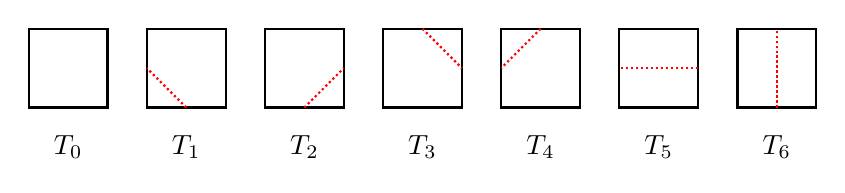
\begin{tikzpicture}
        \cell{0}{0}{1}{1}
        \( \lablnode{0.5}{-0.5}{$T_0$} \) 
        \cellA{1.5}{0}{2.5}{1}
        \( \lablnode{2}{-0.5}{$T_1$} \) 
        \cellB{3}{0}{4}{1}
        \( \lablnode{3.5}{-0.5}{$T_2$} \) 
        \cellC{4.5}{0}{5.5}{1}
        \( \lablnode{5}{-0.5}{$T_3$} \) 
        \cellD{6}{0}{7}{1}
        \( \lablnode{6.5}{-0.5}{$T_4$} \) 
        \cellE{7.5}{0}{8.5}{1}
        \( \lablnode{8}{-0.5}{$T_5$} \) 
        \cellF{9}{0}{10}{1}
        \( \lablnode{9.5}{-0.5}{$T_6$} \) 
    \end{tikzpicture}
\end{center}
\caption{The tile set $\mathbb{T}$}
\label{fig:tile set}
\end{figure}

We denote the set of tiles $\mathbb{T}=\{T_0, \dots, T_{6}\}$. The task is complete once you place $mn$ randomly selected tiles from $\mathbb{T}$ to cover the floor, after which you remove your blindfold. We are interested in the probability of constructing at least one polygon with the red lines with this process.

\begin{figure}[h!]
    \begin{center}
    \begin{subfigure}{0.4\textwidth}
        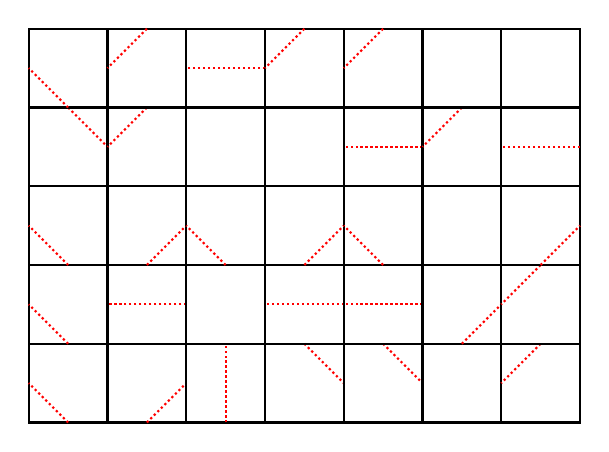
\begin{tikzpicture}
        % row1
        \cellA{0}{0}{1}{1}
        \cellB{1}{0}{2}{1}
        \cellF{2}{0}{3}{1}
        \cellC{3}{0}{4}{1}
        \cellC{4}{0}{5}{1}
        \cell{5}{0}{6}{1}
        \cellD{6}{0}{7}{1}
        % row2
        \cellA{0}{1}{1}{2}
        \cellE{1}{1}{2}{2}
        \cell{2}{1}{3}{2}
        \cellE{3}{1}{4}{2}
        \cellE{4}{1}{5}{2}
        \cellB{5}{1}{6}{2}
        \cellD{6}{1}{7}{2}
        % row3
        \cellA{0}{2}{1}{3}
        \cellB{1}{2}{2}{3}
        \cellA{2}{2}{3}{3}
        \cellB{3}{2}{4}{3}
        \cellA{4}{2}{5}{3}
        \cell{5}{2}{6}{3}
        \cellB{6}{2}{7}{3}
        % row4
        \cellC{0}{3}{1}{4}
        \cellD{1}{3}{2}{4}
        \cell{2}{3}{3}{4}
        \cell{3}{3}{4}{4}
        \cellE{4}{3}{5}{4}
        \cellD{5}{3}{6}{4}
        \cellE{6}{3}{7}{4}
        % row5
        \cellA{0}{4}{1}{5}
        \cellD{1}{4}{2}{5}
        \cellE{2}{4}{3}{5}
        \cellD{3}{4}{4}{5}
        \cellD{4}{4}{5}{5}
        \cell{5}{4}{6}{5}
        \cell{6}{4}{7}{5}
        \end{tikzpicture}
    \caption{A mosaic}
    \label{fig:example mosaic}
    \end{subfigure}
% \hfill
\hspace{0.05\textwidth}
\begin{subfigure}{0.4\textwidth}
    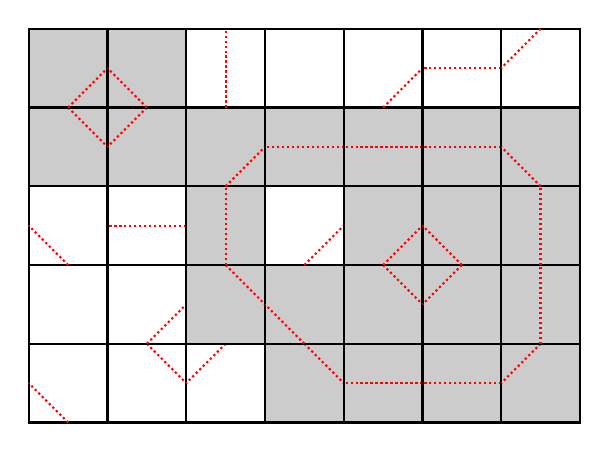
\begin{tikzpicture}
        % row1
        \cellA{0}{0}{1}{1}
        \cellC{1}{0}{2}{1}
        \cellD{2}{0}{3}{1}
        \cellCf{3}{0}{4}{1}
        \cellEf{4}{0}{5}{1}
        \cellEf{5}{0}{6}{1}
        \cellDf{6}{0}{7}{1}
        % row2
        \cell{0}{1}{1}{2}
        \cellB{1}{1}{2}{2}
        \cellCf{2}{1}{3}{2}
        \cellAf{3}{1}{4}{2}
        \cellCf{4}{1}{5}{2}
        \cellDf{5}{1}{6}{2}
        \cellFf{6}{1}{7}{2}
        % row3
        \cellA{0}{2}{1}{3}
        \cellE{1}{2}{2}{3}
        \cellFf{2}{2}{3}{3}
        \cellB{3}{2}{4}{3}
        \cellBf{4}{2}{5}{3}
        \cellAf{5}{2}{6}{3}
        \cellFf{6}{2}{7}{3}
        % row4
        \cellCf{0}{3}{1}{4}
        \cellDf{1}{3}{2}{4}
        \cellBf{2}{3}{3}{4}
        \cellEf{3}{3}{4}{4}
        \cellEf{4}{3}{5}{4}
        \cellEf{5}{3}{6}{4}
        \cellAf{6}{3}{7}{4}
        % row5
        \cellBf{0}{4}{1}{5}
        \cellAf{1}{4}{2}{5}
        \cellF{2}{4}{3}{5}
        \cell{3}{4}{4}{5}
        \cellB{4}{4}{5}{5}
        \cellE{5}{4}{6}{5}
        \cellD{6}{4}{7}{5}
    \end{tikzpicture}
    \caption{A messy polygon mosaic}
    \label{fig:example messy polygon mosaic}
\end{subfigure}

\end{center}
\caption{Examples of mosaics of size $(5,7)$ made of tiles in $\mathbb{T}$}
\label{fig:example mosaics}
\end{figure}

We call a fully tiled $m \times n$ floor an $(m,n)$ \textit{mosaic}. If $m=5$ and $n=7$, you may have constructed the mosaic in Figure \ref{fig:example mosaic}. You may have also constructed the mosaic in Figure \ref{fig:example messy polygon mosaic}. Notice that in the mosaic in Figure \ref{fig:example messy polygon mosaic}, the red dotted lines form multiple polygons\footnote{Polygons are more commonly referred to as ``self-avoiding polygons" in the literature to highlight their connection with self-avoiding walks.}, which we highlight the corresponding tiles in gray. 

\begin{definition}
An $(m,n)$ \textit{messy polygon mosaic} is an $(m,n)$ mosaic that contains at least one polygon. 
\end{definition}

As there are $|\mathbb{T}|^{mn} = 7^{mn}$ total mosaics, we focus on the number of messy polygon mosaics. In fact, it turns out to be simpler to enumerate the number of mosaics that \textit{do not} contain a polygon. Therefore, let $\mathbb{P}^{(m,n)}$ be the subset of $(m,n)$ mosaics that do not contain a polygon. Clearly the number of $(m,n)$ messy polygon mosaics is then $7^{mn} - \left|\mathbb{P}^{(m,n)}\right|$.

From the fact that the smallest polygon is made of $4$ tiles (appearing twice in Figure \ref{fig:example messy polygon mosaic}), we can conclude that $\left|\mathbb{P}^{(n,1)}\right|=7^n$, and $\left|\mathbb{P}^{(2,2)}\right| = 7^4 - 1$. For $m, n \geq 2$, we first define the following matrices.

\begin{definition}

For integers $k \geq 1$ let $A_k, B_k, C_k, D_k$ be $2^{k-1} \times 2^{k-1}$ matrices with integer entries, where $A_{1}=\begin{pmatrix}7\end{pmatrix}, B_{1}=\begin{pmatrix}-1\end{pmatrix}, C_{1}=\begin{pmatrix}1\end{pmatrix}, D_{1}=\begin{pmatrix}1\end{pmatrix}$ and

\begin{eqnarray*}
A_{k+1} = \begin{pmatrix} 7A_{k} & B_{k} \\ C_{k} & D_{k} \end{pmatrix} & B_{k+1} = \begin{pmatrix} -A_{k} & B_{k} \\ 0C_{k} & D_{k} \end{pmatrix} \\
C_{k+1} = \begin{pmatrix} A_{k} & 0B_{k} \\ C_{k} & D_{k} \end{pmatrix} & D_{k+1} = \begin{pmatrix} A_{k} & -B_{k} \\ C_{k} & 7D_{k} \end{pmatrix}.
\end{eqnarray*}
\label{def: matrix defs}
\end{definition}

For matrices, mosaics, and later binary lattices, we number the rows $0,1,\dots,m-1$ top to bottom, and columns $0,1,\dots,n-1$ left to right. Here is our main result.

\begin{thm}
\label{thm: messy mosaics}
The number of $(m,n)$ mosaics that do not contain a polygon $\left|\mathbb{P}^{(m,n)}\right|$ is the $(0,0)$ entry of $A_{n}^m$.
\end{thm}

\section{Related Work}

Hong and Oh \cite{Hong2018} studied a similar question in which they construct mosaics from $\mathbb{T}$, but were interested in the number of polygon mosaics.

\begin{definition}
An $(m,n)$ \textit{polygon mosaic} is an $(m,n)$ mosaic that contains at least one polygon and every tile that is not part of a polygon is $T_0$.
\end{definition}

Clearly, all polygon mosaics are messy polygon mosaics. The sequence A181245 on the OEIS \cite{oeis} is the array of $1 +$ the number of $(m,n)$ polygon mosaics. The authors in \cite{Hong2018} provide bounds for the number of polygon mosaics.

\begin{thm}[\cite{Hong2018}]
\label{thm:Hong2018}
The number of $(m,n)$ polygon mosaics for $m,n \geq 3$ is bounded between
$2^{m+n-3}\left(\frac{17}{10}\right)^{(m-2)(n-2)}$ and $2^{m+n-3}\left(\frac{31}{16}\right)^{(m-2)(n-2)}.$
\end{thm}

In related work, Lomonaco and Kauffman \cite{Lomonaco08} introduced mosaics constructed from a tile set of $11$ distinct tiles, of which $\mathbb{T}$ is a subset. The authors were interested in a subset of mosaics which they call \textit{knot mosaics}. Oh et al. \cite{Oh2014} enumerated the number of knot mosaics.

\begin{thm}[\cite{Oh2014}]
\label{thm:Oh2014}
The number of $(m,n)$ knot mosaics for $m,n \geq 2$ is $2 \left\| (X_{m-2}+O_{m-2})^{n-2} \right\|$, where $X_0 = O_0 = \begin{bmatrix} 1 \\ \end{bmatrix}$ and $X_{m-2}$ and $O_{m-2}$ are $2^{m-2} \times 2^{m-2}$ matrices defined as

$$ X_{k+1} = \begin{pmatrix}
    X_k & O_k \\
    O_k & X_k
\end{pmatrix}
\text{ and }
O_{k+1} = \begin{pmatrix}
    O_k & X_k \\
    X_k & 4O_k
\end{pmatrix}, $$

for $k=0,1,\dots,m-3$. Here $\left\| N \right\|$ denotes the sum of elements of matrix $N$.
\end{thm}

Oh and colleagues go beyond enumeration by bounding the growth rate of knot mosaics \cite{Oh2016, Oh2019, Choi2024}, and Oh further adapts the matrix recursion method to solve problems in monomer and dimer tilings \cite{Oh2018Aztec, Oh2019tiling}. Related ideas were independently used to enumerate the number of rectangular partitions of a rectangle in \cite{oeispaper} for the sequence A182275 on the OEIS \cite{oeis}.

Our work can be seen as an extension to Hong and Oh \cite{Hong2018} and further generalizing the techniques in Oh et al. \cite{Oh2014} to explore a new direction in mosaic enumeration.

\section{Preliminaries}

We begin by defining a map that takes an $(m,n)$ mosaic and gives an $(m,n)$ binary lattice. An $(m,n)$ binary lattice is a rectangular lattice of $m+1$ by $n+1$ vertices, with each vertex labeled $0$ or $1$. We also define a \textit{framed binary lattice} to be a binary lattice in which the boundary vertices are labeled $0$. An example of a $(5,7)$ framed binary lattice is shown on the right of Figure \ref{fig:example of f mapping}.

\begin{definition}

Let $f$ be the map that takes an $(m,n)$ mosaic and labels each vertex with the following rule. If the vertex is surrounded by the red dotted lines of an even number of polygons (including $0$ polygons), label it $0$. If the vertex is surrounded by the red dotted lines of an odd number of polygons, label it $1$. Removing the red dotted lines from the tiles gives the framed binary lattice. 
    
\end{definition}

\begin{figure}[h!]
\begin{center}
    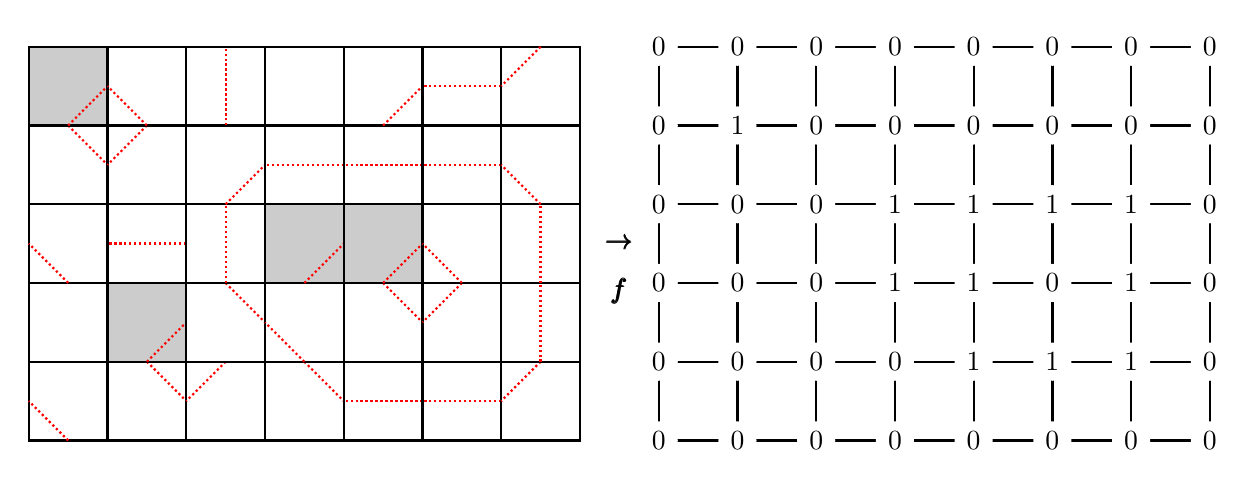
\begin{tikzpicture}
        % row1
        \cellA{0}{0}{1}{1}
        \cellC{1}{0}{2}{1}
        \cellD{2}{0}{3}{1}
        \cellC{3}{0}{4}{1}
        \cellE{4}{0}{5}{1}
        \cellE{5}{0}{6}{1}
        \cellD{6}{0}{7}{1}
        % row2
        \cell{0}{1}{1}{2}
        \cellBf{1}{1}{2}{2}
        \cellC{2}{1}{3}{2}
        \cellA{3}{1}{4}{2}
        \cellC{4}{1}{5}{2}
        \cellD{5}{1}{6}{2}
        \cellF{6}{1}{7}{2}
        % row3
        \cellA{0}{2}{1}{3}
        \cellE{1}{2}{2}{3}
        \cellF{2}{2}{3}{3}
        \cellBf{3}{2}{4}{3}
        \cellBf{4}{2}{5}{3}
        \cellA{5}{2}{6}{3}
        \cellF{6}{2}{7}{3}
        % row4
        \cellC{0}{3}{1}{4}
        \cellD{1}{3}{2}{4}
        \cellB{2}{3}{3}{4}
        \cellE{3}{3}{4}{4}
        \cellE{4}{3}{5}{4}
        \cellE{5}{3}{6}{4}
        \cellA{6}{3}{7}{4}
        % row5
        \cellBf{0}{4}{1}{5}
        \cellA{1}{4}{2}{5}
        \cellF{2}{4}{3}{5}
        \cell{3}{4}{4}{5}
        \cellB{4}{4}{5}{5}
        \cellE{5}{4}{6}{5}
        \cellD{6}{4}{7}{5}
        % arrow
        \( \lablnode{7.5}{2.5}{$\pmb{\to}$} \)
        % 
        \( \lablnode{7.5}{1.9}{$\pmb{f}$} \)

        % row1
        \cell{8}{0}{9}{1}
        \cell{9}{0}{10}{1}
        \cell{10}{0}{11}{1}
        \cell{11}{0}{12}{1}
        \cell{12}{0}{13}{1}
        \cell{13}{0}{14}{1}
        \cell{14}{0}{15}{1}
        % row2
        \cell{8}{1}{9}{2}
        \cell{9}{1}{10}{2}
        \cell{10}{1}{11}{2}
        \cell{11}{1}{12}{2}
        \cell{12}{1}{13}{2}
        \cell{13}{1}{14}{2}
        \cell{14}{1}{15}{2}
        % row3
        \cell{8}{2}{9}{3}
        \cell{9}{2}{10}{3}
        \cell{10}{2}{11}{3}
        \cell{11}{2}{12}{3}
        \cell{12}{2}{13}{3}
        \cell{13}{2}{14}{3}
        \cell{14}{2}{15}{3}
        % row4
        \cell{8}{3}{9}{4}
        \cell{9}{3}{10}{4}
        \cell{10}{3}{11}{4}
        \cell{11}{3}{12}{4}
        \cell{12}{3}{13}{4}
        \cell{13}{3}{14}{4}
        \cell{14}{3}{15}{4}
        % row5
        \cell{8}{4}{9}{5}
        \cell{9}{4}{10}{5}
        \cell{10}{4}{11}{5}
        \cell{11}{4}{12}{5}
        \cell{12}{4}{13}{5}
        \cell{13}{4}{14}{5}
        \cell{14}{4}{15}{5}

        % label for row1
        \( \lablvertex{8}{0}{$0$} \)
        \( \lablvertex{9}{0}{$0$} \)
        \( \lablvertex{10}{0}{$0$} \)
        \( \lablvertex{11}{0}{$0$} \)
        \( \lablvertex{12}{0}{$0$} \)
        \( \lablvertex{13}{0}{$0$} \)
        \( \lablvertex{14}{0}{$0$} \)
        \( \lablvertex{15}{0}{$0$} \)
        % label for row1
        \( \lablvertex{8}{1}{$0$} \)
        \( \lablvertex{9}{1}{$0$} \)
        \( \lablvertex{10}{1}{$0$} \)
        \( \lablvertex{11}{1}{$0$} \)
        \( \lablvertex{12}{1}{$1$} \)
        \( \lablvertex{13}{1}{$1$} \)
        \( \lablvertex{14}{1}{$1$} \)
        \( \lablvertex{15}{1}{$0$} \)
        % label for row1
        \( \lablvertex{8}{2}{$0$} \)
        \( \lablvertex{9}{2}{$0$} \)
        \( \lablvertex{10}{2}{$0$} \)
        \( \lablvertex{11}{2}{$1$} \)
        \( \lablvertex{12}{2}{$1$} \)
        \( \lablvertex{13}{2}{$0$} \)
        \( \lablvertex{14}{2}{$1$} \)
        \( \lablvertex{15}{2}{$0$} \)
        % label for row1
        \( \lablvertex{8}{3}{$0$} \)
        \( \lablvertex{9}{3}{$0$} \)
        \( \lablvertex{10}{3}{$0$} \)
        \( \lablvertex{11}{3}{$1$} \)
        \( \lablvertex{12}{3}{$1$} \)
        \( \lablvertex{13}{3}{$1$} \)
        \( \lablvertex{14}{3}{$1$} \)
        \( \lablvertex{15}{3}{$0$} \)
        % label for row1
        \( \lablvertex{8}{4}{$0$} \)
        \( \lablvertex{9}{4}{$1$} \)
        \( \lablvertex{10}{4}{$0$} \)
        \( \lablvertex{11}{4}{$0$} \)
        \( \lablvertex{12}{4}{$0$} \)
        \( \lablvertex{13}{4}{$0$} \)
        \( \lablvertex{14}{4}{$0$} \)
        \( \lablvertex{15}{4}{$0$} \)
        % label for row1
        \( \lablvertex{8}{5}{$0$} \)
        \( \lablvertex{9}{5}{$0$} \)
        \( \lablvertex{10}{5}{$0$} \)
        \( \lablvertex{11}{5}{$0$} \)
        \( \lablvertex{12}{5}{$0$} \)
        \( \lablvertex{13}{5}{$0$} \)
        \( \lablvertex{14}{5}{$0$} \)
        \( \lablvertex{15}{5}{$0$} \)

    \end{tikzpicture}
\end{center}
\caption{$f$ applied to the mosaic in Figure \ref{fig:example messy polygon mosaic}, resulting in a binary lattice. We highlight each possible way a $T_2$ tile can map to a cell by shading a representative tile in gray.}
\label{fig:example of f mapping}
\end{figure}

To enumerate $|\mathbb{P}^{(m,n)}|$, it will be useful to consider how $f$ maps the tiles in $\mathbb{T}$ to the cells in a binary lattice.

\begin{definition}
Let a \textit{cell} be a $(1,1)$ binary lattice.
\end{definition}

\begin{exmp}
\label{exmp: tile to cell}
Applying $f$ to the mosaic in Figure \ref{fig:example of f mapping} results in the $T_2$ tile at position $(0,0)$ mapping to the cell at position $(0,0)$, diagrammed below.

\begin{center}
    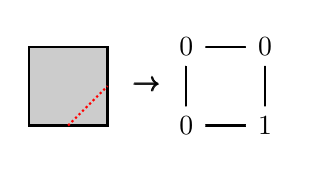
\begin{tikzpicture}
        \cellBf{0}{0}{1}{1}
        
        \( \lablnode{1.5}{0.5}{$\pmb{\to}$} \)
        \cell{2}{0}{3}{1}
        
        \( \lablvertex{2}{0}{$0$} \)
        \( \lablvertex{2}{1}{$0$} \)
        \( \lablvertex{3}{0}{$1$} \)
        \( \lablvertex{3}{1}{$0$} \)
    \end{tikzpicture}
\end{center}

Figure \ref{fig:example of f mapping} also illustrates the three other cells $T_2$ can map to. We diagram applying $f$ to the $T_2$ cells at positions $(2, 3), (2, 4)$, and $(3,1)$ below.

\begin{center}
    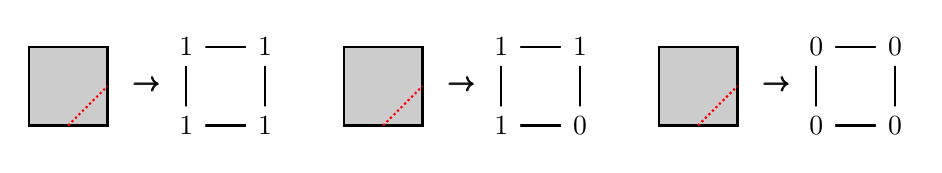
\begin{tikzpicture}
        \cellBf{0}{0}{1}{1}
        \( \lablnode{1.5}{0.5}{$\pmb{\to}$} \)
        \cell{2}{0}{3}{1}
        \( \lablvertex{2}{0}{$1$} \)
        \( \lablvertex{2}{1}{$1$} \)
        \( \lablvertex{3}{0}{$1$} \)
        \( \lablvertex{3}{1}{$1$} \)
        
        \cellBf{4}{0}{5}{1}
        \( \lablnode{5.5}{0.5}{$\pmb{\to}$} \)
        \cell{6}{0}{7}{1}
        \( \lablvertex{6}{0}{$1$} \)
        \( \lablvertex{6}{1}{$1$} \)
        \( \lablvertex{7}{0}{$0$} \)
        \( \lablvertex{7}{1}{$1$} \)
        
        \cellBf{8}{0}{9}{1}
        \( \lablnode{9.5}{0.5}{$\pmb{\to}$} \)
        \cell{10}{0}{11}{1}
        \( \lablvertex{10}{0}{$0$} \)
        \( \lablvertex{10}{1}{$0$} \)
        \( \lablvertex{11}{0}{$0$} \)
        \( \lablvertex{11}{1}{$0$} \)

    \end{tikzpicture}
\end{center}

\end{exmp}

For convenience, we denote a cell by the $2 \times 2$ matrix of its vertex labels. For example, we denote the cell in Example \ref{exmp: tile to cell} as $\begin{smallmatrix} 0 & 0 \\ 0 & 1 \end{smallmatrix}$. There are sixteen cells:  
$$\begin{smallmatrix} 0 & 0 \\ 0 & 0 \end{smallmatrix}, \begin{smallmatrix} 0 & 0 \\ 0 & 1 \end{smallmatrix}, \begin{smallmatrix} 0 & 0 \\ 1 & 0 \end{smallmatrix}, \begin{smallmatrix} 0 & 0 \\ 1 & 1 \end{smallmatrix},\begin{smallmatrix} 0 & 1 \\ 0 & 0 \end{smallmatrix}, \begin{smallmatrix} 0 & 1 \\ 0 & 1 \end{smallmatrix},\begin{smallmatrix} 0 & 1 \\ 1 & 0 \end{smallmatrix}, \begin{smallmatrix} 0 & 1 \\ 1 & 1 \end{smallmatrix},\begin{smallmatrix} 1 & 0 \\ 0 & 0 \end{smallmatrix}, \begin{smallmatrix} 1 & 0 \\ 0 & 1 \end{smallmatrix},\begin{smallmatrix} 1 & 0 \\ 1 & 0 \end{smallmatrix}, \begin{smallmatrix} 1 & 0 \\ 1 & 1 \end{smallmatrix},\begin{smallmatrix} 1 & 1 \\ 0 & 0 \end{smallmatrix}, \begin{smallmatrix} 1 & 1 \\ 0 & 1 \end{smallmatrix},\begin{smallmatrix} 1 & 1 \\ 1 & 0 \end{smallmatrix}, \text{ and }\begin{smallmatrix} 1 & 1 \\ 1 & 1 \end{smallmatrix}.$$

Under $f$, no tile can map to $\begin{smallmatrix} 0 & 1 \\ 1 & 0 \end{smallmatrix}$ or $\begin{smallmatrix} 1 & 0 \\ 0 & 1 \end{smallmatrix}$. Furthermore, tiles that do not form a polygon must map to cells $\begin{smallmatrix} 0 & 0 \\ 0 & 0 \end{smallmatrix}$ or $\begin{smallmatrix} 1 & 1 \\ 1 & 1 \end{smallmatrix}$, and any tile that is part of a polygon must map to one of the twelve remaining possible cells.

We can then define a general function $v$ that maps a cell to some integer, then extend $v$ to $(m,n)$ binary lattices by taking the product over $v$ of the $mn$ individual cells in the binary lattice. We choose the following definition for $v$.

\begin{definition}
Define a map $v$ from cells to integers as follows.

$$\begin{cases}
    7 & \text{for cells } \begin{smallmatrix} 0 & 0 \\ 0 & 0 \end{smallmatrix}, \begin{smallmatrix} 1 & 1 \\ 1 & 1 \end{smallmatrix}\\
    0 & \text{for cells } \begin{smallmatrix} 0 & 1 \\ 1 & 0 \end{smallmatrix}, \begin{smallmatrix} 1 & 0 \\ 0 & 1 \end{smallmatrix}\\
    -1 & \text{for cells } \begin{smallmatrix} 0 & 0 \\ 1 & 0 \end{smallmatrix}, \begin{smallmatrix} 1 & 0 \\ 1 & 1 \end{smallmatrix}\\
    1 & \text{otherwise}
\end{cases}$$

More generally, we define $v$ from binary lattices to integers by taking the product of $v$ applied to each cell in the binary lattice. By definition, $v$ applied to a binary lattice with no cells equals $1$.

\label{def: def of v}
\end{definition}

\begin{exmp}
\label{exmp: v on a ell}
If we let $\ell$ be the framed binary lattice on the right of Figure \ref{fig:example of f mapping}, we have $v(\ell) = -7^{11}$, as there are $2$ $\begin{smallmatrix} 0 & 0 \\ 1 & 0 \end{smallmatrix}$ cells, $1$ $\begin{smallmatrix} 1 & 1 \\ 0 & 1 \end{smallmatrix}$ cells, $9$ $\begin{smallmatrix} 0 & 0 \\ 0 & 0 \end{smallmatrix}$ cells, and $2$ $\begin{smallmatrix} 1 & 1 \\ 1 & 1 \end{smallmatrix}$ cells.
\end{exmp}

We show our choice of $v$ has useful properties by first considering the magnitude, then the sign.  For the magnitude of $v$, for fixed $m,n$ give an index $1 \leq i \leq N$ to every way one polygon can be formed in an $(m,n)$ mosaic. We remind the reader that a polygon is determined not only by its shape and orientation, but also its location within the mosaic. For example, Figure \ref{fig: polygons in different places} depicts three distinct polygons in a $(2,4)$ mosaic, which for reference we call polygons $1, 2,$ and $3$.

\begin{figure}[h!]
\begin{center}
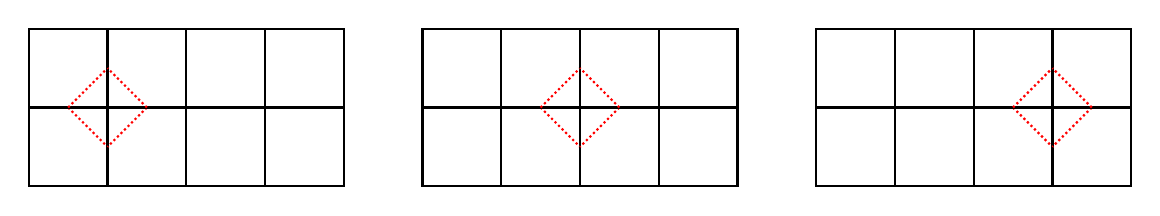
\begin{tikzpicture}
%
\cellC{0}{0}{1}{1}
\cellD{1}{0}{2}{1}
\cell{2}{0}{3}{1}
\cell{3}{0}{4}{1}

\cellB{0}{1}{1}{2}
\cellA{1}{1}{2}{2}
\cell{2}{1}{3}{2}
\cell{3}{1}{4}{2}
%
\cell{5}{0}{6}{1}
\cellC{6}{0}{7}{1}
\cellD{7}{0}{8}{1}
\cell{8}{0}{9}{1}

\cell{5}{1}{6}{2}
\cellB{6}{1}{7}{2}
\cellA{7}{1}{8}{2}
\cell{8}{1}{9}{2}
%
\cell{10}{0}{11}{1}
\cell{11}{0}{12}{1}
\cellC{12}{0}{13}{1}
\cellD{13}{0}{14}{1}

\cell{10}{1}{11}{2}
\cell{11}{1}{12}{2}
\cellB{12}{1}{13}{2}
\cellA{13}{1}{14}{2}

\end{tikzpicture}
\end{center}
\caption{Polygons $1,2,$ and $3$}
\label{fig: polygons in different places}
\end{figure}

\begin{definition}
Let $M_i$ be the set of $(m,n)$ mosaics that contain polygon $i$. 
\label{defn: def of M_i}
\end{definition}

We immediately have the number of messy polygon mosaics is

\begin{equation}
7^{mn} - \Big|\mathbb{P}^{(m,n)}\Big| = \Big|\bigcup_{i=1}^N M_i \Big|.
\label{eq: inc exl setup}
\end{equation}

Notice that not every subset of polygons $1 \leq i \leq N$ has a mosaic that contains them all. For example, for the polygons in Figure \ref{fig: polygons in different places} the second-from-left column contains different tiles in polygon $1$ and polygon $2$, so no mosaic exists that contain these two polygons. Consequently $M_1 \cap M_2 = \varnothing$.

\begin{prop}
Let $J$ be a subset of indices of polygons. If there exists at least one mosaic that contains all polygons in $J$, we have

\begin{equation}
\Big|\bigcap_{j \in J} M_j \Big| = \Big|v(\ell)\Big|,
\label{eq: intersect of M}
\end{equation}

\noindent where $\ell$ is the framed binary lattice such that $\ell = f(\mathcal{M})$ where $\mathcal{M}$ is any mosaic that only contains the polygons in $J$.
\label{prop: mag of v}
\end{prop}

\begin{proof}
From the definition of $M_j$, the left hand side of Equation \ref{eq: intersect of M} counts the number of mosaics that necessarily contain the polygons in $J$, and possibly contain other polygons. For the right hand side, if a cell comes from a tile that is part of a polygon, the absolute value of $v$ of the cell is $1$. Therefore, $|v(\ell)|$ is just $7$ to the number of $\begin{smallmatrix} 0 & 0 \\ 0 & 0 \end{smallmatrix}$ and $\begin{smallmatrix} 1 & 1 \\ 1 & 1 \end{smallmatrix}$ cells in $\ell$. As all tiles in $\mathbb{T}$ can map to $\begin{smallmatrix} 0 & 0 \\ 0 & 0 \end{smallmatrix}$ and $\begin{smallmatrix} 1 & 1 \\ 1 & 1 \end{smallmatrix}$, $|v(\ell)|$ counts all possible tile assignments in all locations that are not part of a polygon in $J$. Therefore $|v(\ell)|$ counts mosaics that contain the polygons in $J$. This is the definition of $\bigcap_{i \in S} M_i$, and so the equality holds.
\end{proof}

\begin{definition}
If $\ell$ is a framed binary lattice that does not contain $\begin{smallmatrix} 0 & 1 \\ 1 & 0 \end{smallmatrix}$ or $\begin{smallmatrix} 1 & 0 \\ 0 & 1 \end{smallmatrix}$, let $P(\ell)$ to be the number of polygons in the polygon mosaic formed by replacing all $\begin{smallmatrix} 0 & 0 \\ 0 & 0 \end{smallmatrix}$ and $\begin{smallmatrix} 1 & 1 \\ 1 & 1 \end{smallmatrix}$ cells with the blank tile $T_0$, and replacing all other cells with the unique tile that maps to that cell under $f$.
\end{definition}

For the sign of $v$, we show that though $v(\ell)$ is computed ``cell-by-cell'', we recover global information about $P(\ell)$.

\begin{prop} 
If $\ell$ is a framed binary lattice that does not contain the cells $\begin{smallmatrix} 0 & 1 \\ 1 & 0 \end{smallmatrix}$ or $\begin{smallmatrix} 1 & 0 \\ 0 & 1 \end{smallmatrix}$, then 
\begin{equation}
    \text{sign}(v(\ell)) = (-1)^{P(\ell)}.
\label{eq: sign prop}
\end{equation}
\label{prop: sign of v}
\end{prop}

\begin{proof}

For this proof, we use LHS and RHS to abbreviate the left and right hand side of Equation \ref{eq: sign prop}. We prove the result by induction. For the base case, construct the $(0,n)$ framed binary lattice $\ell$ for some $n \geq 0$. As there are no cells in $\ell$, from the definition of $v$ the LHS is $\text{sign}(v(\ell))=1$. As there no polygons in $g(\ell)$, we have the RHS is $1$.

For the induction step, consider any $(m+1,n)$ framed binary strip $\ell'$ for $m \geq 1$ such that there are no $\begin{smallmatrix} 0 & 1 \\ 1 & 0 \end{smallmatrix}$ or $\begin{smallmatrix} 1 & 0 \\ 0 & 1 \end{smallmatrix}$ cells. Similarly, define $\ell$ to be the framed binary lattice that shares the top $m$ rows of vertices with $\ell'$, and the bottom most row all being $0$. We show that we can construct $\ell'$ from $\ell$ with a procedure that preserves Equation \ref{eq: sign prop} with each intermediate step.

\noindent\textbf{Procedure:} \\
\indent \textbf{Step 1.} Add a bottom row to $\ell$ of $n+1$ vertices, all labeled $0$. This results in a new $(m+1,n)$ framed binary lattice we denote $\ell_1$. \\
\indent \textbf{Step 2.} Scanning rows $m-1$ and $m$ of $\ell'$ left to right, if there exists a column of the form $\begin{smallmatrix} 1 \\ 1 \end{smallmatrix}$, change the associated $\begin{smallmatrix} 1 \\ 0 \end{smallmatrix}$ column in $\ell_1$ to $\begin{smallmatrix} 1 \\ 1 \end{smallmatrix}$. Completing this scan results in a new framed binary lattice denoted $\ell_2$.\\
\indent \textbf{Step 3.} Again scanning rows $m-1$ and $m$ of $\ell'$ left to right, if there exists a column of the form $\begin{smallmatrix} 0 \\ 1 \end{smallmatrix}$, change the associated $\begin{smallmatrix} 0 \\ 0 \end{smallmatrix}$ column in $\ell_2$ to $\begin{smallmatrix} 0 \\ 1 \end{smallmatrix}$. Completing this scan results in the framed binary lattice $\ell'$.\\

For step 1, only $\begin{smallmatrix} 0 & 0 \\ 0 & 0 \end{smallmatrix}$ cells are added. As $\text{sign}\left(v\left(\begin{smallmatrix} 0 & 0 \\ 0 & 0 \end{smallmatrix}\right)\right) = 1$, the LHS is unchanged. For the RHS no new polygons are created in $g(\ell_1)$, so Equation \ref{eq: sign prop} is preserved by step 1.

For steps 2 and 3, we prove the result for each intermediate vertex change as we scan left to right. Furthermore, as each intermediate change only flips a single vertex label from $0$ to $1$, we only need to consider the $4$ cells that share this vertex. We diagram all possible cases for both steps in Figure \ref{fig: step 2 cases} and Figure \ref{fig: step 3 cases}, where the \# symbol indicates the vertex flipping from a $0$ to a $1$. We know that the bottom most row of vertices must all be $0$ by construction.

For step 2, the vertex above the \# symbol must be $1$ by definition. Also, the vertex right of the \# symbol must be $0$, as the procedure moves left to right on $\ell_1$. Additionally, the $\begin{smallmatrix} 0 & 1 \\ 1 & 0 \end{smallmatrix}$ cell cannot be created or destroyed, and so Figure \ref{fig: step 2 cases} depicts all $6$ possible cases.

\begin{figure}[h!]
\centering
\begin{subfigure}[t]{0.2\textwidth}
\begin{center}
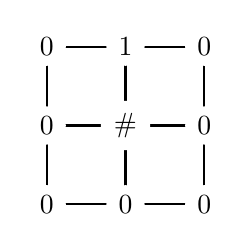
\begin{tikzpicture}
% row 1 of cells
\cell{0}{0}{1}{1}
\cell{1}{0}{2}{1}
\cell{0}{-1}{1}{0}
\cell{1}{-1}{2}{0}
% row 1 labels
\( \lablvertex{0}{0}{$0$} \)
\( \lablvertex{1}{0}{\#} \)
\( \lablvertex{2}{0}{$0$} \)
% row 2 labels
\( \lablvertex{0}{1}{$0$} \)
\( \lablvertex{1}{1}{$1$} \)
\( \lablvertex{2}{1}{$0$} \)
% row -1 labels
\( \lablvertex{0}{-1}{$0$} \)
\( \lablvertex{1}{-1}{$0$} \)
\( \lablvertex{2}{-1}{$0$} \)
\end{tikzpicture}
\end{center}
\caption{}
\label{subfig: step 2 bit flip case 1}
\end{subfigure}
~
\begin{subfigure}[t]{0.2\textwidth}
\begin{center}
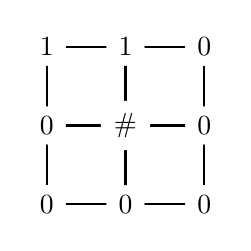
\begin{tikzpicture}
% row 1 of cells
\cell{0}{0}{1}{1}
\cell{1}{0}{2}{1}
\cell{0}{-1}{1}{0}
\cell{1}{-1}{2}{0}
% row 1 labels
\( \lablvertex{0}{0}{$0$} \)
\( \lablvertex{1}{0}{\#} \)
\( \lablvertex{2}{0}{$0$} \)
% row 2 labels
\( \lablvertex{0}{1}{$1$} \)
\( \lablvertex{1}{1}{$1$} \)
\( \lablvertex{2}{1}{$0$} \)
% row -1 labels
\( \lablvertex{0}{-1}{$0$} \)
\( \lablvertex{1}{-1}{$0$} \)
\( \lablvertex{2}{-1}{$0$} \)
\end{tikzpicture}
\end{center}
\caption{}
\label{subfig: step 2 bit flip case 2}
\end{subfigure}
~
\begin{subfigure}[t]{0.2\textwidth}
\begin{center}
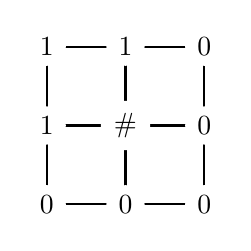
\begin{tikzpicture}
% row 1 of cells
\cell{0}{0}{1}{1}
\cell{1}{0}{2}{1}
\cell{0}{-1}{1}{0}
\cell{1}{-1}{2}{0}
% row 1 labels
\( \lablvertex{0}{0}{$1$} \)
\( \lablvertex{1}{0}{\#} \)
\( \lablvertex{2}{0}{$0$} \)
% row 2 labels
\( \lablvertex{0}{1}{$1$} \)
\( \lablvertex{1}{1}{$1$} \)
\( \lablvertex{2}{1}{$0$} \)
% row -1 labels
\( \lablvertex{0}{-1}{$0$} \)
\( \lablvertex{1}{-1}{$0$} \)
\( \lablvertex{2}{-1}{$0$} \)
\end{tikzpicture}
\end{center}
\caption{}
\label{subfig: step 2 bit flip case 3}
\end{subfigure}

% \hfill

\begin{subfigure}[t]{0.2\textwidth}
\begin{center}
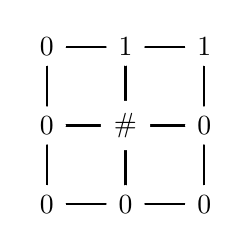
\begin{tikzpicture}
% row 1 of cells
\cell{0}{0}{1}{1}
\cell{1}{0}{2}{1}
\cell{0}{-1}{1}{0}
\cell{1}{-1}{2}{0}
% row 1 labels
\( \lablvertex{0}{0}{$0$} \)
\( \lablvertex{1}{0}{\#} \)
\( \lablvertex{2}{0}{$0$} \)
% row 2 labels
\( \lablvertex{0}{1}{$0$} \)
\( \lablvertex{1}{1}{$1$} \)
\( \lablvertex{2}{1}{$1$} \)
% row -1 labels
\( \lablvertex{0}{-1}{$0$} \)
\( \lablvertex{1}{-1}{$0$} \)
\( \lablvertex{2}{-1}{$0$} \)
\end{tikzpicture}
\end{center}
\caption{}
\label{subfig: step 2 bit flip case 4}
\end{subfigure}
~
\begin{subfigure}[t]{0.2\textwidth}
\begin{center}
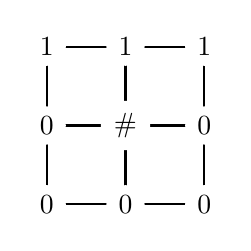
\begin{tikzpicture}
% row 1 of cells
\cell{0}{0}{1}{1}
\cell{1}{0}{2}{1}
\cell{0}{-1}{1}{0}
\cell{1}{-1}{2}{0}
% row 1 labels
\( \lablvertex{0}{0}{$0$} \)
\( \lablvertex{1}{0}{\#} \)
\( \lablvertex{2}{0}{$0$} \)
% row 2 labels
\( \lablvertex{0}{1}{$1$} \)
\( \lablvertex{1}{1}{$1$} \)
\( \lablvertex{2}{1}{$1$} \)
% row -1 labels
\( \lablvertex{0}{-1}{$0$} \)
\( \lablvertex{1}{-1}{$0$} \)
\( \lablvertex{2}{-1}{$0$} \)
\end{tikzpicture}
\end{center}
\caption{}
\label{subfig: step 2 bit flip case 5}
\end{subfigure}
~
\begin{subfigure}[t]{0.2\textwidth}
\begin{center}
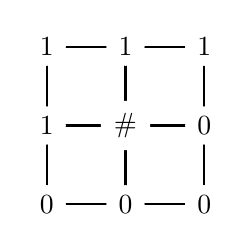
\begin{tikzpicture}
% row 1 of cells
\cell{0}{0}{1}{1}
\cell{1}{0}{2}{1}
\cell{0}{-1}{1}{0}
\cell{1}{-1}{2}{0}
% row 1 labels
\( \lablvertex{0}{0}{$1$} \)
\( \lablvertex{1}{0}{\#} \)
\( \lablvertex{2}{0}{$0$} \)
% row 2 labels
\( \lablvertex{0}{1}{$1$} \)
\( \lablvertex{1}{1}{$1$} \)
\( \lablvertex{2}{1}{$1$} \)
% row -1 labels
\( \lablvertex{0}{-1}{$0$} \)
\( \lablvertex{1}{-1}{$0$} \)
\( \lablvertex{2}{-1}{$0$} \)
\end{tikzpicture}
\end{center}
\caption{}
\label{subfig: step 2 bit flip case 6}
\end{subfigure}
\caption{Step 2 Cases}
\label{fig: step 2 cases}
\end{figure}

\noindent As no case in Figure \ref{fig: step 2 cases} creates or destroys any $\begin{smallmatrix} 0 & 0 \\ 1 & 0 \end{smallmatrix}$ or $\begin{smallmatrix} 1 & 0 \\ 1 & 1 \end{smallmatrix}$ cells, the LHS sign does not change for any intermediate vertex flip. Similarly, one can check that both before and after the vertex is changed from $0$ to $1$ that the following is true. Replacing each $\begin{smallmatrix} 0 & 0 \\ 0 & 0 \end{smallmatrix}$ and $\begin{smallmatrix} 1 & 1 \\ 1 & 1 \end{smallmatrix}$ cell with $T_0$ and replacing all other cells with their unique corresponding tile only forms tiles that must all be part of the same polygon. For example, the corresponding tiles for Case \ref{subfig: step 2 bit flip case 5} is shown in Figure \ref{fig: step 2 example tile swap}.

\begin{figure}[h!]
\centering
\begin{subfigure}[t]{0.2\textwidth}
\begin{center}
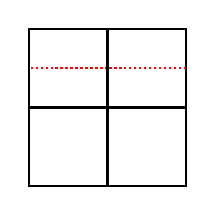
\begin{tikzpicture}
% row 1 of cells
\cell{0}{0}{1}{1}
\cell{1}{0}{2}{1}
% row 2 of cells
\cellE{0}{1}{1}{2}
\cellE{1}{1}{2}{2}
\end{tikzpicture}
\end{center}
\end{subfigure}
~
\begin{subfigure}[t]{0.2\textwidth}
\begin{center}
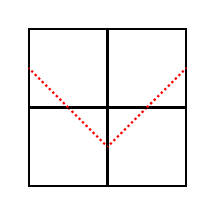
\begin{tikzpicture}
% row 1 of cells
\cellC{0}{0}{1}{1}
\cellD{1}{0}{2}{1}
% row 2 of cells
\cellA{0}{1}{1}{2}
\cellB{1}{1}{2}{2}
\end{tikzpicture}
\end{center}
\end{subfigure}
\caption{Tile configurations before and after flipping the vertex in Case \ref{subfig: step 2 bit flip case 5}}
\label{fig: step 2 example tile swap}
\end{figure}

\noindent Therefore the number of polygons remains the same, and so the RHS is preserved.

For step 3, the vertex above the \# symbol must be $0$ by definition. As we cannot create or destroy $\begin{smallmatrix} 0 & 1 \\ 1 & 0 \end{smallmatrix}$ or $\begin{smallmatrix} 1 & 0 \\ 0 & 1 \end{smallmatrix}$ cells, Figure \ref{fig: step 3 cases} depicts all $6$ possible cases.

\begin{figure}[h!]
\centering
\begin{subfigure}[t]{0.2\textwidth}
\begin{center}
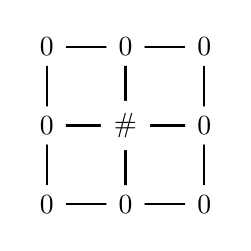
\begin{tikzpicture}
% row 1 of cells
\cell{0}{0}{1}{1}
\cell{1}{0}{2}{1}
\cell{0}{-1}{1}{0}
\cell{1}{-1}{2}{0}
% row 1 labels
\( \lablvertex{0}{0}{$0$} \)
\( \lablvertex{1}{0}{\#} \)
\( \lablvertex{2}{0}{$0$} \)
% row 2 labels
\( \lablvertex{0}{1}{$0$} \)
\( \lablvertex{1}{1}{$0$} \)
\( \lablvertex{2}{1}{$0$} \)
% row -1 labels
\( \lablvertex{0}{-1}{$0$} \)
\( \lablvertex{1}{-1}{$0$} \)
\( \lablvertex{2}{-1}{$0$} \)
\end{tikzpicture}
\end{center}
\caption{}
\label{subfig: bit flip case 1}
\end{subfigure}
~
\begin{subfigure}[t]{0.2\textwidth}
\begin{center}
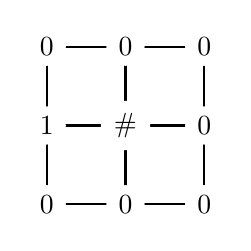
\begin{tikzpicture}
% row 1 of cells
\cell{0}{0}{1}{1}
\cell{1}{0}{2}{1}
\cell{0}{-1}{1}{0}
\cell{1}{-1}{2}{0}
% row 1 labels
\( \lablvertex{0}{0}{$1$} \)
\( \lablvertex{1}{0}{\#} \)
\( \lablvertex{2}{0}{$0$} \)
% row 2 labels
\( \lablvertex{0}{1}{$0$} \)
\( \lablvertex{1}{1}{$0$} \)
\( \lablvertex{2}{1}{$0$} \)
% row -1 labels
\( \lablvertex{0}{-1}{$0$} \)
\( \lablvertex{1}{-1}{$0$} \)
\( \lablvertex{2}{-1}{$0$} \)
    
\end{tikzpicture}
\end{center}
\caption{}
\label{subfig: bit flip case 2}
\end{subfigure}
~
\begin{subfigure}[t]{0.2\textwidth}
\begin{center}
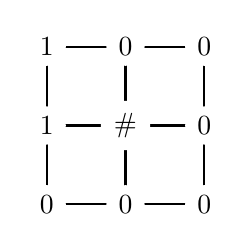
\begin{tikzpicture}
% row 1 of cells
\cell{0}{0}{1}{1}
\cell{1}{0}{2}{1}
\cell{0}{-1}{1}{0}
\cell{1}{-1}{2}{0}
% row 1 labels
\( \lablvertex{0}{0}{$1$} \)
\( \lablvertex{1}{0}{\#} \)
\( \lablvertex{2}{0}{$0$} \)
% row 2 labels
\( \lablvertex{0}{1}{$1$} \)
\( \lablvertex{1}{1}{$0$} \)
\( \lablvertex{2}{1}{$0$} \)
% row -1 labels
\( \lablvertex{0}{-1}{$0$} \)
\( \lablvertex{1}{-1}{$0$} \)
\( \lablvertex{2}{-1}{$0$} \)
\end{tikzpicture}
\end{center}
\caption{}
\label{subfig: bit flip case 3}
\end{subfigure}

% \hfill

\begin{subfigure}[t]{0.2\textwidth}
\begin{center}
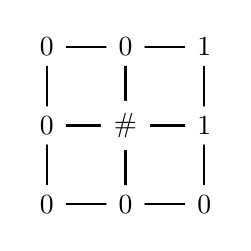
\begin{tikzpicture}
% row 1 of cells
\cell{0}{0}{1}{1}
\cell{1}{0}{2}{1}
\cell{0}{-1}{1}{0}
\cell{1}{-1}{2}{0}
% row 1 labels
\( \lablvertex{0}{0}{$0$} \)
\( \lablvertex{1}{0}{\#} \)
\( \lablvertex{2}{0}{$1$} \)
% row 2 labels
\( \lablvertex{0}{1}{$0$} \)
\( \lablvertex{1}{1}{$0$} \)
\( \lablvertex{2}{1}{$1$} \)
% row -1 labels
\( \lablvertex{0}{-1}{$0$} \)
\( \lablvertex{1}{-1}{$0$} \)
\( \lablvertex{2}{-1}{$0$} \)
\end{tikzpicture}
\end{center}
\caption{}
\label{subfig: bit flip case 4}
\end{subfigure}
~
\begin{subfigure}[t]{0.2\textwidth}
\begin{center}
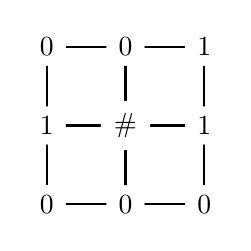
\begin{tikzpicture}
% row 1 of cells
\cell{0}{0}{1}{1}
\cell{1}{0}{2}{1}
\cell{0}{-1}{1}{0}
\cell{1}{-1}{2}{0}
% row 1 labels
\( \lablvertex{0}{0}{$1$} \)
\( \lablvertex{1}{0}{\#} \)
\( \lablvertex{2}{0}{$1$} \)
% row 2 labels
\( \lablvertex{0}{1}{$0$} \)
\( \lablvertex{1}{1}{$0$} \)
\( \lablvertex{2}{1}{$1$} \)
% row -1 labels
\( \lablvertex{0}{-1}{$0$} \)
\( \lablvertex{1}{-1}{$0$} \)
\( \lablvertex{2}{-1}{$0$} \)
\end{tikzpicture}
\end{center}
\caption{}
\label{subfig: bit flip case 5}
\end{subfigure}
~
\begin{subfigure}[t]{0.2\textwidth}
\begin{center}
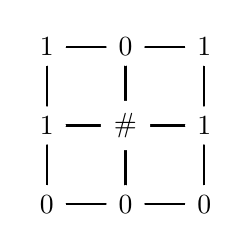
\begin{tikzpicture}
% row 1 of cells
\cell{0}{0}{1}{1}
\cell{1}{0}{2}{1}
\cell{0}{-1}{1}{0}
\cell{1}{-1}{2}{0}
% row 1 labels
\( \lablvertex{0}{0}{$1$} \)
\( \lablvertex{1}{0}{\#} \)
\( \lablvertex{2}{0}{$1$} \)
% row 2 labels
\( \lablvertex{0}{1}{$1$} \)
\( \lablvertex{1}{1}{$0$} \)
\( \lablvertex{2}{1}{$1$} \)
% row -1 labels
\( \lablvertex{0}{-1}{$0$} \)
\( \lablvertex{1}{-1}{$0$} \)
\( \lablvertex{2}{-1}{$0$} \)
\end{tikzpicture}
\end{center}
\caption{}
\label{subfig: bit flip case 6}
\end{subfigure}
\caption{Step 3 Cases}
\label{fig: step 3 cases}
\end{figure}

We show Equation \ref{eq: sign prop} holds case by case. In Case \ref{subfig: bit flip case 1}, the flip add one $\begin{smallmatrix} 0 & 0 \\ 1 & 0 \end{smallmatrix}$ cell, so the sign of the LHS changes. As the flip creates a new polygon the sign of the RHS changes. In Case \ref{subfig: bit flip case 2}, the flip removes and adds a $\begin{smallmatrix} 0 & 0 \\ 1 & 0 \end{smallmatrix}$ cell, so the sign of the LHS stays the same. As the flip does not create a new polygon, the RHS stays the same. In Case \ref{subfig: bit flip case 3}, the flip adds both a $\begin{smallmatrix} 0 & 0 \\ 1 & 0 \end{smallmatrix}$ cell and a $\begin{smallmatrix} 1 & 0 \\ 1 & 1 \end{smallmatrix}$ cell, so the sign of the LHS stays the same. As the flip does not create a new polygon, the RHS stays the same. In Case \ref{subfig: bit flip case 4}, the flip does not add a $\begin{smallmatrix} 0 & 0 \\ 1 & 0 \end{smallmatrix}$ cell or $\begin{smallmatrix} 1 & 0 \\ 1 & 1 \end{smallmatrix}$ cell, so the sign of the LHS stays the same. As the flip does not create a new polygon, the RHS stays the same. In Case \ref{subfig: bit flip case 5}, the flip removes a $\begin{smallmatrix} 0 & 0 \\ 1 & 0 \end{smallmatrix}$ cell, so the sign of the LHS changes. Before the flip, replacing the cells with the appropriate tiles results in a configuration that can either represent portions of one or two polygons, as shown in Figure \ref{fig: tile config for double case}.

\begin{figure}[h!]
\centering
\begin{subfigure}[t]{0.2\textwidth}
\begin{center}
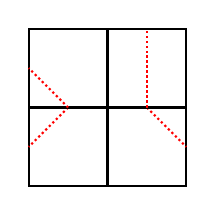
\begin{tikzpicture}
% row 1 of cells
\cellD{0}{0}{1}{1}
\cellC{1}{0}{2}{1}
% row 2 of cells
\cellA{0}{1}{1}{2}
\cellF{1}{1}{2}{2}
\end{tikzpicture}
\end{center}
\end{subfigure}
~
\begin{subfigure}[t]{0.2\textwidth}
\begin{center}
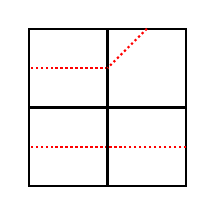
\begin{tikzpicture}
% row 1 of cells
\cellE{0}{0}{1}{1}
\cellE{1}{0}{2}{1}
% row 2 of cells
\cellE{0}{1}{1}{2}
\cellD{1}{1}{2}{2}
\end{tikzpicture}
\end{center}
\end{subfigure}
\caption{Tile configurations before and after flipping the vertex in Case \ref{subfig: bit flip case 5}}
\label{fig: tile config for double case}
\end{figure}

\noindent If the tiles were part of one polygon before the flip, the tiles after the flip must be part of two distinct polygons. Similarly, if the tiles are were part of two polygons before the flip, the tiles after the flip must be of one polygon. Either way the total number of polygons changes by $1$, and so the RHS changes sign. In Case \ref{subfig: bit flip case 6}, the flip adds $\begin{smallmatrix} 1 & 0 \\ 1 & 1 \end{smallmatrix}$, so the sign of the LHS changes. The same logic from Case \ref{subfig: bit flip case 5} applies for the RHS, as the flip either removes or adds a polygon.

As all cases preserve Equation \ref{eq: sign prop}, the $(m+1, n)$ framed binary lattice $\ell'$ also follows Equation \ref{eq: sign prop}.
\end{proof}

\begin{thm}
The number of $(m,n)$ mosaics that do not contain a polygon has
\begin{equation}
\left|\mathbb{P}^{(m,n)}\right| = \sum_{\ell} v(\ell),
\label{eq: sum of v}
\end{equation}
where the sum is over all $(m,n)$ framed binary lattices.
\label{thm: sum of vs}
\end{thm}

\begin{proof}

We begin by rewriting Equation \ref{eq: inc exl setup} to 

$$\Big|\mathbb{P}^{(m,n)}\Big| = 7^{mn} - \Big|\bigcup_{i=1}^N M_i \Big|.$$

By the inclusion-exclusion principle, we have

\begin{equation}
-\Big|\bigcup_{i=1}^N M_i \Big| = \sum_{\varnothing \neq J \subseteq \{1,2,\dots,N\}}(-1)^{|J|}\Big|\bigcap_{j \in J} M_j \Big|.
\label{eq: incl excl applied}
\end{equation}

Consider an individual subset of polygon indices $J$ in the sum in Equation \ref{eq: incl excl applied} such that $|J|=k \geq 1$. If there exists no mosaic that contains all polygons in $J$, by the definition of $M$ the term is $0$. If at least one mosaic does exist, Propositions \ref{prop: mag of v} and \ref{prop: sign of v} give the following

$$(-1)^{|J|}\Big|\bigcap_{j \in J} M_j \Big| = v(\ell),$$

where $\ell$ is the binary lattice such that $f(\mathcal{M}) = \ell$ for all mosaics $\mathcal{M}$ that contain at least the polygons in $J$.

Now discard all $0$ terms in Equation \ref{eq: incl excl applied} and group the terms in Equation \ref{eq: incl excl applied} for all $J$ such that $|J|=k$. From the definition of $M$, the absolute value of this collection of terms counts the number of mosaics that have at least $k$ polygons, and so

$$\sum_{J \subseteq \{1,2,\dots,N\}, |J|=k}(-1)^{|J|}\Big|\bigcap_{j \in J} M_j \Big| = \sum_{\{\ell | P(\ell) = k\}}v(\ell).$$

Additionally notice that the binary lattice $\ell^*$ made up of all $\begin{smallmatrix} 0 & 0 \\ 0 & 0 \end{smallmatrix}$ cells has $v(\ell^*) = 7^{mn}$, and is the only framed binary lattice such that $P(\ell) = 0$. Therefore, we can write

$$\Big|\mathbb{P}^{(m,n)}\Big| = 7^{mn} - \Big|\bigcup_{i=1}^N M_i \Big| = \sum_{k \geq 0} \sum_{\{\ell | P(\ell) = k\}}v(\ell).$$

Finally, notice that the sum $\sum_{\ell}v(\ell) = 0$ for the framed binary lattices that contains $\begin{smallmatrix} 0 & 1 \\ 1 & 0 \end{smallmatrix}$ or $\begin{smallmatrix} 1 & 0 \\ 0 & 1 \end{smallmatrix}$, as $v\left(\begin{smallmatrix} 0 & 1 \\ 1 & 0 \end{smallmatrix}\right)=v\left(\begin{smallmatrix} 1 & 0 \\ 0 & 1 \end{smallmatrix}\right)=0$. Therefore, summing over all framed binary lattices in Equation \ref{eq: sum of v} gives the desired result.
\end{proof}

As in Theorem \ref{thm:Oh2014} from \cite{Oh2014}, we can compute the sum in Equation \ref{eq: sum of v} efficiently using the matrix recursion method, which we describe next.

\section{Proof of Theorem \ref{thm: messy mosaics}}

We begin by recognizing the matrices $A_k, B_k, C_k, D_k$ in Definition \ref{def: matrix defs} can be rewritten using any function $v$ from cells to integers that is extended to $(m,n)$ binary lattices as the product over individual cells. We write $A_{1}=\begin{pmatrix}v(\begin{smallmatrix} 0 & 0 \\ 0 & 0 \end{smallmatrix})\end{pmatrix}, B_{1}=\begin{pmatrix}v(\begin{smallmatrix} 0 & 0 \\ 1 & 0 \end{smallmatrix})\end{pmatrix}, C_{1}=\begin{pmatrix}v(\begin{smallmatrix} 1 & 0 \\ 0 & 0 \end{smallmatrix})\end{pmatrix}, D_{1}=\begin{pmatrix}v(\begin{smallmatrix} 1 & 0 \\ 1 & 0 \end{smallmatrix})\end{pmatrix}$, and for integers $k \geq 1$,

\begin{eqnarray*}
A_{k+1} = \begin{pmatrix} v(\begin{smallmatrix} 0 & 0 \\ 0 & 0 \end{smallmatrix})A_{k} & v(\begin{smallmatrix} 0 & 0 \\ 0 & 1 \end{smallmatrix})B_{k} \\ v(\begin{smallmatrix} 0 & 1 \\ 0 & 0 \end{smallmatrix})C_{k} & v(\begin{smallmatrix} 0 & 1 \\ 0 & 1 \end{smallmatrix})D_{k} \end{pmatrix} & B_{k+1} = \begin{pmatrix} v(\begin{smallmatrix} 0 & 0 \\ 1 & 0 \end{smallmatrix})A_{k} & v(\begin{smallmatrix} 0 & 0 \\ 1 & 1 \end{smallmatrix})B_{k} \\ v(\begin{smallmatrix} 0 & 1 \\ 1 & 0 \end{smallmatrix})C_{k} & v(\begin{smallmatrix} 0 & 1 \\ 1 & 1 \end{smallmatrix})D_{k} \end{pmatrix} \\
C_{k+1} = \begin{pmatrix} v(\begin{smallmatrix} 1 & 0 \\ 0 & 0 \end{smallmatrix})A_{k} & v(\begin{smallmatrix} 1 & 0 \\ 0 & 1 \end{smallmatrix})B_{k} \\ v(\begin{smallmatrix} 1 & 1 \\ 0 & 0 \end{smallmatrix})C_{k} & v(\begin{smallmatrix} 1 & 1 \\ 0 & 1 \end{smallmatrix})D_{k} \end{pmatrix} & D_{k+1} = \begin{pmatrix} v(\begin{smallmatrix} 1 & 0 \\ 1 & 0 \end{smallmatrix})A_{k} & v(\begin{smallmatrix} 1 & 0 \\ 1 & 1 \end{smallmatrix})B_{k} \\ v(\begin{smallmatrix} 1 & 1 \\ 1 & 0 \end{smallmatrix})C_{k} & v(\begin{smallmatrix} 1 & 1 \\ 1 & 1 \end{smallmatrix})D_{k} \end{pmatrix}.
\end{eqnarray*}

We work with general $v$ in this section, and substitute the specific $v$ from Definition \ref{def: def of v} to give Theorem \ref{thm: messy mosaics}, as well as exactly enumerating the number of polygon mosaics that were bounded in \cite{Hong2018}.

\begin{definition}
Let the $n$ digit binary representation of the number $k$ be written as $\beta_n(k)$. If $n$ is $0$, $\beta_n(k)$ returns the empty string.
\end{definition}

We extend our shorthand for cells to $(1,n)$ binary lattice using analagous matrix notation and the definition for $\beta_n(k)$. For example, we write

$$v\left(\begin{smallmatrix} 0 & \beta_{2}(1) & 0 \\ 0 & \beta_{2}(0) & 0 \end{smallmatrix}\right) = v \Big(\begin{smallmatrix} 0 & 0 & 1 & 0 \\ 0 & 0 & 0 & 0 \end{smallmatrix}\Big) = v \Big(\begin{smallmatrix} 0 & 0 \\ 0 & 0 \end{smallmatrix}\Big) v \Big(\begin{smallmatrix} 0 & 1 \\ 0 & 0 \end{smallmatrix}\Big) v \Big(\begin{smallmatrix} 1 & 0 \\ 0 & 0 \end{smallmatrix}\Big).$$

Finally, we remind the reader matrix elements are indexed starting at $0$.

\begin{prop}
For all integers $n \geq 1$, the $(i,j)$-th entry of \begin{eqnarray*}
A_n \text{ is } v\left(\begin{smallmatrix} 0 & \beta_{n-1}(i) & 0 \\ 0 & \beta_{n-1}(j) & 0 \end{smallmatrix}\right), & B_n \text{ is } v\left(\begin{smallmatrix} 1 & \beta_{n-1}(i) & 0 \\ 0 & \beta_{n-1}(j) & 0 \end{smallmatrix}\right), \\
C_n \text{ is } v\left(\begin{smallmatrix} 0 & \beta_{n-1}(i) & 0 \\ 1 & \beta_{n-1}(j) & 0 \end{smallmatrix}\right), & D_n \text{ is } v\left(\begin{smallmatrix} 1 & \beta_{n-1}(i) & 0 \\ 1 & \beta_{n-1}(j) & 0 \end{smallmatrix}\right).
\end{eqnarray*}
\label{prop: one by n matrix}
\end{prop}

\begin{proof}
We prove by induction. The $n=1$ case is trivial, as $\beta_0(0)$ is the empty string. We next assume our result for some fixed $n \geq 1$. Since $A_n$ has size $2^{n-1} \times 2^{n-1}$, the $(i, j+2^{n-1})$ element of $A_{n+1}$ equals $v\left(\begin{smallmatrix} 0 & 0 \\ 0 & 1 \end{smallmatrix}\right)$ times the $(i,j)$ element of $B_n$. By our induction hypothesis, this equals

$$v\Big(\begin{smallmatrix} 0 & 0 \\ 0 & 1 \end{smallmatrix}\Big)v\left(\begin{smallmatrix} 0 & \beta_{n-1}(i) & 0 \\ 1 & \beta_{n-1}(j) & 0 \end{smallmatrix}\right) = v\left(\begin{smallmatrix} 0 & 0 & \beta_{n-1}(i) & 0 \\ 0 & 1 & \beta_{n-1}(j) & 0 \end{smallmatrix}\right) = v\left(\begin{smallmatrix} 0 & \beta_{n}(i) & 0 \\ 0 & \beta_{n}(j+2^{n-1}) & 0 \end{smallmatrix}\right),$$

\noindent as desired. Analagous arguments show that the other blocks in $A_{n+1}$ have the desired values. Similarly, since $C_n$ has size $2^{n-1} \times 2^{n-1}$, the $(i+2^{n-1}, j)$ element of $D_{n+1}$ equals $v\left(\begin{smallmatrix} 1 & 1 \\ 1 & 0 \end{smallmatrix}\right)$ times the $(i,j)$ element of $C_n$. By our induction hypothesis, this equals

$$v\Big(\begin{smallmatrix} 1 & 1 \\ 1 & 0 \end{smallmatrix}\Big)v\left(\begin{smallmatrix} 1 & \beta_{n-1}(i) & 0 \\ 0 & \beta_{n-1}(j) & 0 \end{smallmatrix}\right) = v\left(\begin{smallmatrix} 1 & 1 & \beta_{n-1}(i) & 0 \\ 1 & 0 & \beta_{n-1}(j) & 0 \end{smallmatrix}\right) = v\left(\begin{smallmatrix} 1 & \beta_{n}(i+2^{n-1}) & 0 \\ 1 & \beta_{n}(j) & 0 \end{smallmatrix}\right),$$

\noindent again as desired. These arguments must be adapted to prove the desired results for all blocks of $B_{n+1}, C_{n+1},$ and $D_{n+1}$, but all the work is similar. 
\end{proof}

We further extend our shorthand for binary lattices. If an $m,n$ binary lattices $\ell$ has the top row of vertices $0\beta_{n-1}(i)0$ and the bottom row of vertices $0\beta_{n-1}(j)0$, and the left and right-most column of vertices being labeled $0$, we write $\ell$ is like $\begin{smallmatrix} 0 & \beta_{n-1}(i) & 0 \\ & \dots & \\ 0 & \beta_{n-1}(j) & 0 \end{smallmatrix}.$

\begin{prop}
For all positive integers $m,n$, the $(i,j)$-th entry of $A^{m}_{n}$ is $\sum v(\ell)$, where the sum is over all $(m, n)$ binary lattices like $\begin{smallmatrix} 0 & \beta_{n-1}(i) & 0 \\ & \dots & \\ 0 & \beta_{n-1}(j) & 0 \end{smallmatrix}$.
\label{prop: m by n matrix}
\end{prop}

\begin{proof}
We prove by induction. The base case $m=1$ is Proposition \ref{prop: one by n matrix}, as the sum is only over $\begin{smallmatrix} 0 & \beta_{n-1}(i) & 0 \\ 0 & \beta_{n-1}(j) & 0 \end{smallmatrix}$. We next assume our result for fixed positive $m,n$. From the induction hypothesis, for any integer $k \in \{0,1,\dots,2^{n-1}-1\}$ the $(i, k)$-th entry of $A_n$ is $v\Big(\begin{smallmatrix} 0 & \beta_{n-1}(i) & 0 \\ 0 & \beta_{n-1}(k) & 0 \end{smallmatrix}\Big)$ and the $(k,j)$-th entry of $A^{m}_{n}$ is

$$\sum_{\ell \text{ like } \begin{smallmatrix} 0 & \beta_{n-1}(k) & 0 \\ & \dots & \\ 0 & \beta_{n-1}(j) & 0 \end{smallmatrix}} v\left(\ell\right).$$

The $(i,j)$-th element of $A_{n} \cdot A^{m}_n$ is the dot product of the $i$-th row of $A_{n}$ and the $j$-th column of $A^{m}_n$. By construction, that is

$$\sum_{k=0}^{2^{n-1}-1} v\left(\begin{smallmatrix} 0 & \beta_{n-1}(i) & 0 \\ 0 & \beta_{n-1}(k) & 0 \end{smallmatrix}\right) \sum_{\ell \text{ like } \begin{smallmatrix} 0 & \beta_{n-1}(k) & 0 \\ & \dots & \\ 0 & \beta_{n-1}(j) & 0 \end{smallmatrix}} v\left(\ell\right) = \sum_{\ell \text{ like } \begin{smallmatrix} 0 & \beta_{n-1}(i) & 0 \\ & \dots & \\ 0 & \beta_{n-1}(j) & 0 \end{smallmatrix}} v\left(\ell\right),$$

which gives the desired result.
\end{proof}

\noindent \textbf{Theorem \ref{thm: messy mosaics}.} The number of $(m,n)$ mosaics that do not contain a polygon is the $(0,0)$ entry of $A_{n}^m$.

\begin{proof}
By Proposition \ref{prop: m by n matrix}, the $(0,0)$ entry of $A^{m}_{n}$ is $\sum v(\ell)$, where the sum is over all $(m, n)$ binary lattices of the form 

$$\begin{smallmatrix} 0 & \beta_{n-1}(0) & 0 \\ & \dots & \\ 0 & \beta_{n-1}(0) & 0 \end{smallmatrix},$$

\noindent which is simply all framed binary lattices. Substituting the values for $v$ from Definition \ref{def: def of v} gives the sum from Theorem \ref{thm: sum of vs}, which completes the proof.
\end{proof}

Our work immediately gives the number of polygon mosaics considered in \cite{Hong2018}. There is a one-to-one correspondence between polygon mosaics and framed binary lattices that do not contain the cells $\begin{smallmatrix} 0 & 1 \\ 1 & 0 \end{smallmatrix}$ or $\begin{smallmatrix} 1 & 0 \\ 0 & 1 \end{smallmatrix}$, as for polygon mosaics under $f$ the cells $\begin{smallmatrix} 0 & 0 \\ 0 & 0 \end{smallmatrix}$ and $\begin{smallmatrix} 1 & 1 \\ 1 & 1 \end{smallmatrix}$ can only come from the $T_0$ tile. Consequently, we can define $v$ for cells as

$$\begin{cases}
    0 & \text{for cells } \begin{smallmatrix} 0 & 1 \\ 1 & 0 \end{smallmatrix}, \begin{smallmatrix} 1 & 0 \\ 0 & 1 \end{smallmatrix}\\
    1 & \text{otherwise}
\end{cases}$$

\noindent and again extend to binary lattices as the product of $v$ evaluated at individual cells. 

We can then substitute our new definition of $v$ into the definitions for matrices $A_k, B_k, C_k$ and $D_k$ to efficiently compute $\sum_{\ell}v(\ell)$ for some $m,n$. Additionally, the authors in \cite{Hong2018} did not consider the mosaic of all $T_0$ a polygon mosaic. Therefore $v$ of the binary lattice of all $\begin{smallmatrix} 0 & 0 \\ 0 & 0 \end{smallmatrix}$ cells should not be considered in the final sum, and so we have the following result.

\begin{theorem}
The number of polygon mosaics is the $(0,0)$ element of $A_n^m$ minus $1$.
\end{theorem}

We point out that this result is likely known to the authors of \cite{Hong2018} and \cite{Oh2014}, though to our knowledge it has not appeared in print.

\newpage

\printbibliography

% \section{Appendix}

\end{document}